\section{Plan 9}
\label{sec:plan9}

\par What is Plan9 ? A movie from Ed Wood ? A 'new' Operative System ?\textit{Plan9 from Bell Labs} is an Operative System developed \href{http://swtch.com/plan9history/}{between the 80's and 2002} by the research and development subsidiary of the French-owned Alcatel-Lucent in Berkeley Heights, New Jersey, United States.\textit{Yes, the name is from the movie :)}

\begin{figure}[H]
\centering
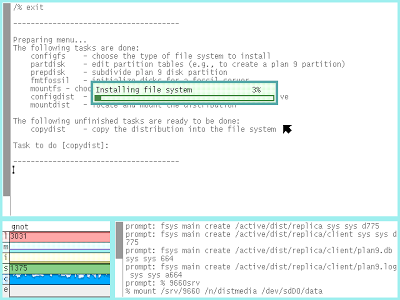
\includegraphics[width=\textwidth]{plan9-install}
\caption{Plan9 talk by \textit{Enrique Soriano Salvador}}
\label{plan9-film}
\end{figure}

\par Plan9 was developed by the same developers of Unix to create a real network OS where \textit{everything} is a file. Even the processes. Everything is related to the basic input/output file readers, the main purpose in the ancient Unix.

\subsection{Technologies}

\textit{Plan9}is developed using C language. The tools they use to collaborate are:
\begin{itemize}
	\item \textit{Mail lists} - to get in touch with the community and contribute tool \url{http://plan9.bell-labs.com/wiki/plan9/mailing_lists}.
	\item \textit{patch} - Command (\href{http://plan9.bell-labs.com/magic/man2html/1/patch}{\textit{patch}})to create file changes.
	\item \textit{Online Sources} -\url{http://plan9.bell-labs.com/sources/}
	\item \textit{TODO} -\url{http://plan9.bell-labs.com/wiki/plan9/TODO/index.html}
	\item \textit{Contrib index} -\url{http://plan9.bell-labs.com/wiki/plan9/Contrib_index/index.html}
	\item \textit{Irc channel} -\url{http://plan9.bell-labs.com/wiki/plan9/IRC/index.html}
	\item \textit{Workshops} - \url{http://www.iwp9.org/}
\end{itemize}

\subsection{How to Contribute}

\par Contributing to the community is difficult, because all your contributions have to pass Plan9 filter handled by one person. You don't depend on a community itself.

\par By other way, you have a very good guidelines and references by very good C developers to \href{http://plan9.bell-labs.com/magic/man2html/6/style}{develop Plan9}.

\begin{itemize}
	\item don't use // comments; some old Plan 9 code does, but we're converting it as we touch it. We do sometimes use // to comment-out a few lines of code.
	\item avoid gotos.
	\item no tabs expanded to spaces.
	\item no white space before opening braces.
	\item no white space after the word "if", "for", "while", etc.
	\item no braces around single-line blocks (e.g., if, for, and while bodies).
	\item integer-valued functions return -1 on error, 0 or positive on success.
	\item functions that return errors should set errstr(2).
	\item variable and function names are all lowercase, with no underscores.
	\item enum or \#defined constants should be Uppercase or UPPERCASE.
	\item struct tags are Uppercase, with matching typedefs.
	\item automatic variables (local variables inside a function) are never initialized at declaration.
	\item follow the standard idioms: use x$<$0 not 0$>$x, etc.
\end{itemize} The end they follow a very common development filosophy:

\begin{quotation}
    \textit{Ultimately, the goal is to write code that fits in with the other code around it and the system as a whole. If the file you are editing already deviates from these guidelines, do what it does. After you edit a file, a reader should not be able to tell just from coding style which parts you worked on.}
\end{quotation}

\par In my opinion, \textit{Plan9 is a very good Operative System to learn how an Operative System works and enjoy learning}.

% section plan9 (end)